\documentclass[a4paper,11pt]{article}
\input{/home/tof/Documents/Cozy/latex-include/preambule_lua.tex}
\newcommand{\showprof}{show them}  % comment this line if you don't want to see todo environment
\fancyhead[L]{TITRE}
\newdate{madate}{10}{09}{2020}
%\fancyhead[R]{\displaydate{madate}} %\today
%\fancyhead[R]{Seconde - SNT}
%\fancyhead[R]{Première - NSI}
\fancyhead[R]{Terminale - NSI}
\fancyfoot[L]{~\\Christophe Viroulaud}
\AtEndDocument{\label{lastpage}}
\fancyfoot[C]{\textbf{Page \thepage/\pageref{lastpage}}}
\fancyfoot[R]{\includegraphics[width=2cm,align=t]{/home/tof/Documents/Cozy/latex-include/cc.png}}

\begin{document}
\begin{Form}
\begin{center}
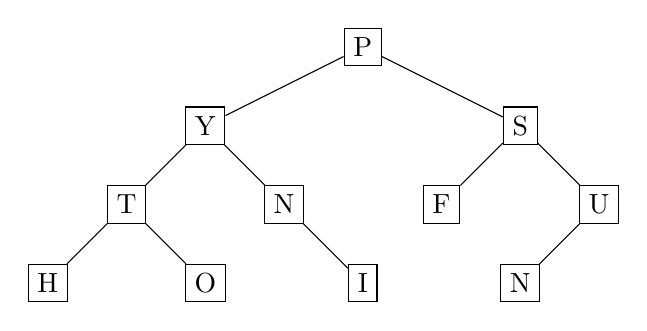
\begin{tikzpicture}
\node[draw] (P) at (0,0) {P};
\node[draw] (Y) at (-2,-1) {Y};
\node[draw] (T) at (-3,-2) {T};
\node[draw] (N) at (-1,-2) {N};
\node[draw] (H) at (-4,-3) {H};
\node[draw] (O) at (-2,-3) {O};
\node[draw] (I) at (0,-3) {I};
\node[draw] (S) at (2,-1) {S};
\node[draw] (F) at (1,-2) {F};
\node[draw] (U) at (3,-2) {U};
\node[draw] (N2) at (2,-3) {N};
\draw (P) -- (Y);
\draw (T) -- (Y);
\draw (T) -- (H);
\draw (T) -- (O);
\draw (N) -- (Y);
\draw (N) -- (I);
\draw (P) -- (S);
\draw (F) -- (S);
\draw (S) -- (U);
\draw (N2) -- (U);
\end{tikzpicture}
\captionof{figure}{Une structure arborescente}
\label{arbre}
\end{center}
\section{Parcours d'un arbre}
Les dossiers d'un système d'exploitation sont construits sous forme d'un arbre. Comme dans un graphe nous pouvons parcourir cet arbre de plusieurs manières, en partant de la racine.
\subsection{Parcours en largeur}
L'arbre est parcouru niveau par niveau. À chaque étage les nœuds sont parcourus de gauche à droite.
\begin{activite}
Parcourir en largeur l'arbre de la figure \ref{arbre}.
\end{activite}
\subsection{Parcours en profondeur}
L'un des deux sous-arbres est parcouru entièrement avant que le second ne soit exploré. On distingue trois types de parcours:
\begin{itemize}
\item \textbf{parcours préfixe:} chaque nœud est visité avant que ses fils le soient,
\item \textbf{parcours infixe:} chaque nœud est visité après son fils gauche mais avant son fils droit,
\item \textbf{parcours postfixe:} chaque nœud est visité après ses fils.
\end{itemize}
\begin{activite}
Réaliser les trois types de parcours pour l'arbre de la figure \ref{arbre}.
\end{activite}
\section{Rechercher un fichier}
La commande \emph{find} du système Linux parcourt les sous-dossiers pour trouver le document demandé.
\\
\begin{activite}
\begin{enumerate}
\item Se rendre sur le simulateur de \emph{terminal Linux}: \url{https://tinyurl.com/y839kd4f} .
\item Créer l'arborescence de dossiers de la figure \ref{arbre} à l'aide des instructions suivantes:
\begin{itemize}
\item Créer le dossier \emph{p}
\begin{lstlisting}
mkdir p
\end{lstlisting}
\item Entre dans le dossier \emph{p}
\begin{lstlisting}
cd p
\end{lstlisting}
\item Retourner dans le dossier père
\begin{lstlisting}
cd ..
\end{lstlisting}
\end{itemize}
\item Se placer dans le dossier \emph{p}.
\item La commande suivante affiche le parcours d'une recherche quelconque. L'exécuter.
\begin{lstlisting}
find -print
\end{lstlisting}
\item Quel type de parcours effectue la fonction \emph{find}?
\end{enumerate}
\end{activite}
\end{Form}
\end{document}